\documentclass[12pt, onecolumn, titlepage]{article}

\usepackage[brazil]{babel}
%\usepackage[latin1]{inputenc}
\usepackage[utf8]{inputenc}
\usepackage{graphicx}
\graphicspath{{figuras/}}
\usepackage{geometry}
%\geometry{
%	a4paper,
%	left=3cm,
%	top=3cm,
%	right=2cm,
%	bottom=2cm
%}
\usepackage{float}

\begin{document} %Inicio do documento

\begin{titlepage} %Capa
	
	\vfill
	\begin{center}
	
		{\large \textbf{Faculdade de Ciências e Tecnologia\\Universidade Estadual Paulista\\``Júlio de Mesquita Filho''}} \\[3cm]
		{\small \textbf{Bruno Santos de Lima - RA: 141251093}}\\
		{\small \textbf{Leandro Ungari Cayres - RA: 141250992}}\\[3cm]
		{\Large Definição do Projeto}\\
		{\Large Sistema FoodExpress}\\[3cm]

	\hspace{.45\textwidth} %posiciona a minipage
	\begin{minipage}{.5\textwidth}
		\small Disciplina de Banco de Dados I. Professor Dr. Ronaldo Celso Messias Correia, pelo curso de Ciência da Computação. Com data de entrega 05 de Junho de 2016 \\[0.5cm]
	\end{minipage}

	\vfill
	\vspace{1.5cm}
	
	\large \textbf{Presidente Prudente\\}
	\large \textbf{Maio - 2016}
	
	\end{center}
	
\end{titlepage}
%Fim da capa
\newpage

\renewcommand{\contentsname}{Índice}
\tableofcontents

\newpage

\section{Introdução}
\label{sect:introducao}

Este documento tem como propósito descrever detalhes referentes ao Sistema FoodExpress, detalhes tanto no quesito de funcionamento do sistema, quanto principalmente em relação a particularidades de caráter técnico relacionados a área de Ciência da Computação com ênfase em Banco de Dados. 

Essa coletânea está dividida como segue: na seção \ref{sect:especificacao} é especificado o sistema bem como sua lógica de funcionamento, na seção \ref{sect:conceitual} é apresentado o modelo entidade relacionamento do sistema, a seção \ref{sect:relacional} mostra o processo de mapeamento para o modelo conceitual e seu respectivo modelo, em seguida a seção \ref{sect:normalizacao} evidencia discussões referentes ao processo de normalização, por fim a seção \ref{sect:algebra} apresenta detalhes pertinentes as principais consultas a serem realizadas e sua resolução utilizando Álgebra Relacional.

\section{Especificação do Problema}
\label{sect:especificacao}

O Sistema FoodExpress consiste em uma ferramenta para gerenciamento de uma distribuidora de alimentos, com o intuito de armazenar os dados necessários para a que a empresa possa realizar a gestão de seus clientes, fornecedores, produtos e rotas de viagens, bem como fornecer um mecanismo que facilite a obtenção dos melhores caminhos para o transporte das mercadorias até as localizações de seus clientes.

No sistema os clientes (empresas e estabelecimentos comerciais do setor alimentício) da distribuidora podem realizar encomendas para serem entregues em seus respectivos estabelecimento, os gerentes da distribuidora devem ter acesso a essas encomendas e utilizam o sistema para elaborar viagens com rotas convenientes em termos de custos de viagem, especificando tipo de carga, veículo e motorista que farão parte desta. O Gerentes da distribuidora também tem controle de todo o sistema de estoque, podendo realizar pedidos aos seus fornecedores (fábricas, produtores rurais, entre outros) para repor o mesmo, ou para atender as necessidades de um cliente em especifico.

A ferramenta consiste em uma plataforma web, implementada utilizando a linguagem de programação PHP, além da utilização da linguagem de marcação e de estilo: HTML e CSS, contendo algumas aplicações de JavaScript, além de utilizar como Sistema Gerenciador de Banco de Dados (SGBD) o MySQL.

\subsection{Entidades}
\label{sect:entidades}

Abaixo segue especificado o conjunto de entidades necessárias para a elaboração deste projeto, todas as entidades estão organizadas com o prefixo E seguido de um número que identifica a mesma de forma única neste documento, além disso cada entidade contém um conjunto de atributos que também estão especificados, observe abaixo:

\begin{description}

\item E1. Funcionario
\item \qquad Atributos: idFuncionario (PK), nome, salario, dataContratacao e dataNascimento.

\item E1.1. Motorista
\item \qquad Atributos: São os mesmos do funcionario, pois é uma entidade especializada contendo ainda os seguintes atributos próprios: idMotorista (PK), categoriaHabilitacao, telefone e disponivel.

\item E1.2. Gerente
\item \qquad Atributos: São os mesmos do funcionario, pois é uma entidade especializada contendo ainda os seguintes atributos próprios: idGerente (PK), email, login e senha.

\item E1.3. Segurança
\item \qquad Atributos: São os mesmos do funcionario, pois é uma entidade especializada contendo ainda os seguintes atributos próprios: idSeguranca (PK) e porteArma.

\item E1.4. AuxiliarLimpeza
\item \qquad Atributos: São os mesmos do funcionario, pois é uma entidade especializada contendo ainda os seguintes atributos próprios: idLimpeza (PK) e setor.

\item E2. Fornecedor
\item \qquad Atributos: cnpj (PK), nome, email e telefone.

\item E2.1. Fabrica
\item \qquad Atributos: São os mesmos do fornecedor, pois é uma entidade especializada, contendo ainda seu atributo próprio: idFrabrica (PK).

\item E2.2. Agricultor
\item \qquad Atributos: São os mesmos do fornecedor, pois é uma entidade especializada, contendo ainda seu atributo próprio: idAgricultor (PK).

\item E2.3. Outro
\item \qquad Atributos: São os mesmos do outro, pois é uma entidade especializada, contendo ainda seu atributo próprio: idOutro (PK).

\item E3. Empresa
\item \qquad Atributos: cnpj (PK), nome, proprietario, chaveAcesso e senha.

\item E4. Produto
\item \qquad Atributos: codProduto (PK), preco, dataFabricacao e dataNascimento.

\item E5. Pedido
\item \qquad Atributos: idPedido (PK),data e status.

\item E6. Deposito
\item \qquad Atributos: numero (PK), descricao e capacidade.

\item E7. Viagem
\item \qquad Atributos: idViagem (PK) e descricao.

\item E8. Veiculo
\item \qquad Atributos: idVeiculo (PK), modelo, placa, ano, capacidade e disponivel.

\item E9. Endereço
\item \qquad Atributos: idEndereco (PK), logradouro, numero, bairro e completo.

\item E10. Cidade
\item \qquad Atributos: idCidade (PK), nome, estado e pais.

\item E11. Pagamento
\item \qquad Atributos: idPagamento (PK), numeroBoleto, descricao, valor e dataVencimento, dataEmissao e status.

\item E12. Item
\item \qquad Atributos: quantidade e precoTotal.

\item E13. Especificação do Produto
\item \qquad Atributos: idEspecProduto (PK), nome e descricao.

\item E14. Encomenda
\item \qquad Atributos: idEncomenda (PK), data e status.

\end{description}

\subsection{Relacionamento entre Entidades}
\label{sect:relacionamento}

Definidas as entidades que serão utilizadas, tem-se a necessidade de especificar os relacionamentos entre essas entidades, cada uma dos relacionamento está exemplificado abaixo:

\begin{description}

\item Gerente \textbf{Faz} Pedido: 
\item \qquad O Gerente (E1.2) da distribuidora de alimentos utiliza o sistema para fazer Pedido (E5) de itens para um de seus fornecedores. O Pedido pode ser feito por um Gerente e um Gerente pode fazer vários pedidos.

%\item Gerente \textbf{Controla} Deposito: 
%\item \qquad O Gerente (E1.2) controla os produtos pertencentes ao Deposito (E6) da distribuidora de alimentos. O Gerente pode %controlar vários Depósitos e os Depósitos podem ser controladores por vários Gerentes.

\item Gerente \textbf{Solicita} Viagem: 
\item \qquad O Gerente (E1.2) da distribuidora de alimentos, ciente da existência de encomendas realizadas por seus clientes, solicita uma Viagem (E7) para a entrega de um conjunto de encomendas. O Gerente pode solicitar várias Viagens, assim como as Viagens podem ser solicitadas por vários Gerentes.

\item Pedido \textbf{Possui} Item: 
\item \qquad O Pedido (E5) no caso está relacionado estritamente com o pedido da distribuidora de alimentos para um de seus fornecedores com o intuito de abastecer o seu deposito de produtos, cada Pedido contém um conjunto de Itens (E12), assim um Pedido pode ter vários Itens, porem cada Item pode estar contido em um único Pedido.

\item Viagem \textbf{Possui} Veiculo: 
\item \qquad Cada uma das Viagens (E7) realizadas, tem como o objetivo entregar encomendas para os clientes da distribuidora de alimentos, assim em cada uma dessas viagens tem-se um Veículo (E8) para realização da mesma. Cada Viagem é realizada por um Veículo e cada Veículo pode realizar várias viagens.

\item Motorista \textbf{Realiza} Viagem: 
\item \qquad O Motorista (E1.1) realiza a Viagem (E7) seguindo uma rota previamente determinada. Um Motorista pode realizar várias Viagens e uma Viagem pode ser realizada por um Motorista.

\item Viagem \textbf{Referente} Encomenda: 
\item \qquad A Viagem (E7) acontece com a finalidade de entregar Encomendas (E14) para os clientes da distribuidora. Uma Viagem pode referir-se a várias Encomendas e uma Encomenda pode estar em uma Viagem.

\item Endereco \textbf{Pertence} Cidade: 
\item \qquad Todos os Endereços (E9) pertencem a uma determinada Cidade (E10). Um Endereço pertence a uma única Cidade, já uma Cidade pode conter diversos Endereços.

\item Empresa \textbf{Localizada} Endereco: 
\item \qquad As Empresas (E3), que são clientes da distribuidora de alimentos, tem endereços físicos, onde esses Endereços (E9) são utilizados para realizar a entrega de encomendas para as Empresas clientes da distribuidora de alimentos. Uma Empresa tem um único Endereço e um Endereço pertence a uma única Empresa.

\item Fornecedor \textbf{Localizado} Endereco: 
\item \qquad Os Fornecedores (E2) da distribuidora de alimentos, tem endereços físicos. Um Fornecedor tem um único Endereço (E9) e um Endereço pertence a um único Fornecedor.

\item Fornecedor \textbf{Fornece} Produto: 
\item \qquad O Fornecedor (E2) é o responsável por suprir as necessidades da distribuidora fornecendo os Produtos (E4) necessários para abastecer o deposito da mesma. Um Fornecedor pode fornecer um ou mais produtos e um produto pode ser fornecido por um ou mais distribuidor.

\item Deposito \textbf{Contem} Produto: 
\item \qquad O Deposito (E6) da distribuidora de alimentos contém uma série de Produtos (E4) que podem ser encomendados pelas Empresas que são clientes. O Deposito pode conter diversos Produtos e cada Produto pode estar em um Deposito.

\item Pagamento \textbf{Refere} Pedido: 
\item \qquad Todo Pedido (E5) realizado por um Gerente da distribuidora de alimentos para um fornecedor deve ter um Pagamento (E11) associado a ele. Todo Pagamento pode ter diversos pedidos, porem cada Pedido deve estar presente em apenas um Pagamento.

\item Pagamento \textbf{Refere} Encomenda: 
\item \qquad Toda Encomenda (E14) realizada por uma empresa cliente da distribuidora de alimentos deve ter um Pagamento (E11) associado a ele. Todo Pagamento pode ter diversas Encomendas, porem cada Encomenda deve estar presente em apenas um Pagamento.

\item EspecificacaoProduto \textbf{refere} Produto: 
\item \qquad Em cada uma das encomendas realizadas pelas empresas clientes da distribuidora de alimentos existe uma Especificação (E13) de um Produto que refere-se a um Produto (E4) disponibilizado pela distribuidora. Neste caso cada Produto tem apenas uma Especificação e vice-versa. 

\item Encomenda \textbf{Contem} EspecificacaoProduto: 
\item \qquad Cada Encomenda (E14) contém contém um conjunto de especificações, cada especificação está ligada a um produto pertencente a Encomenda. Cada Encomenda contém diversas Especificações (E13) de Produto, sendo que está última está presente em diversas Encomendas.

\item Empresa \textbf{Pede} Encomenda: 
\item \qquad A Empresa (E3) cliente da distribuidora de alimentos realiza pedidos de Encomenda (E14) que uma serie de produtos, onde essas Encomendas devem ser entregas pela distribuidora diretamente no endereço da Empresa. Cada Empresa pode realizar pedidos por várias Encomendas e uma Encomenda pode ser pedida por apenas uma Empresa.

\end{description}

\subsection{Principais Consultas}
\label{sect:principaisConsultas}

Dentre as consultas em que o sistema pode realizar no Banco de Dados, podemos destacar dez destas como as principais, observe abaixo:

\begin{enumerate}

\item Listagem de encomendas a partir de uma data.

\item Busca por fornecedores que ofertam um determinado produto.

\item Listagem de pagamentos recebidos de empresas.

\item Listagem de pagamentos realizados a fornecedores.

\item Listagem de encomendas solicitadas.

\item Busca e conseguentemente a listagem de endereços de entrega relativos às encomendas.

\item Listagem de pedidos realizados.

\item Consulta e listagem de veículos disponíveis.

\item Consulta e listagem de motoristas disponíveis.

\item Listagem de pedidos em andamento.

%1 - Verificar se o item está presente em algum depósito.
%1 - Listagem de encomendas a partir de uma data.
%2 - Busca por fornecedores que ofertam um determinado produto
%3 - Listagem de entradas (pagamentos recebidos de empresas)
%4 - Listagem de saídas (pagamentos realizados a fornecedores)
%5 - Listagem de encomendas solicitadas
%6 - Buscar endereços de entrega relativos às encomendas
%7 - Listagem de pedidos realizados
%8 - Consulta a veículos disponíveis
%9 - Consulta a motoristas disponíveis
%10 - Lista de pedidos em andamento

\end{enumerate}

\newpage
\section{Esquema Conceitual}
\label{sect:conceitual}

Com base nas entidades e nas relações entre elas apresentadas anteriormente neste documento na seção \ref{sect:especificacao}, foi modelado o esquema conceitual do projeto para o sistema FoodExpress, este modelo trata-se do modelo entidade-relacionamento, ou simplesmente modelo ER. Este modelo pode ser observado a seguir:

\newpage

\begin{figure}[H]
  \centering
  \includegraphics[scale=0.25, angle=90]{modelo-conceitual.png}
  \label{figRotulo}
\end{figure}

\newpage
\section{Mapeamento do Esquema Relacional}
\label{sect:relacional}
A seguir serão descritas todas as etapas do processo de modelagem do modelo conceitual (ER) para o relacional.

No primeiro passo, para cada entidade no modelo ER são criadas tabelas correspondentes, para os atributos compostos somente são incluídos os atributos simples e deve ser escolhida uma chave primária.
\\
\renewcommand{\baselinestretch}{1.2}
\begin{table}[htb!]
\begin{center}
\begin{tabular}{p{2.5cm} p{10.5cm}}
cidade & (\underline{idCidade}, nome, estado, pais) \\
endereco & (\underline{idEndereco}, logradouro, numero, bairro, complemento) \\
veiculo & (\underline{idVeiculo}, placa, ano, modelo, capacidade, disponivel) \\
viagem & (\underline{idViagem}, descricao) \\
funcionario & (\underline{idFuncionario}, nome, salario, dataContratacao, dataNascimento)\\
motorista & (\underline{idMotorista}, categoriaHabilitacao, codigo, area, numero, disponivel)\\
seguranca & (\underline{idSeguranca}, porteArma)\\
gerente & (\underline{idGerente}, email, login, senha)\\
auxiliarlimpeza & (\underline{idLimpeza}, setor)\\
deposito & (\underline{numero}, descricao, capacidade)\\
pedido & (\underline{idPedido}, dataPedido, status)\\
produto & (\underline{codProduto}, preco, dataFabricacao, dataVencimento)\\
fornecedor & (\underline{cnpj}, nome, email, codigo, area, numero)\\
fabrica & (\underline{idFabrica})\\
agricultor & (\underline{idAgricultor})\\
outro & (\underline{idOutro})\\
pagamento & (\underline{idPagamento}, numeroBoleto, descricao, valor, dataVencimento, dataEmissao)\\
especifproduto & (\underline{idEspecProduto}, nome, descricao)\\
encomenda & (\underline{idEncomenda}, data, status)\\
empresa & (\underline{cnpj}, proprietario, nome, chaveAcesso, senha)
\end{tabular}
\end{center}
\end{table}

No segundo passo, são criadas tabelas para todos as entidades fracas incluindo nestas todos os atributos simples, como há entidades fracas neste modelo, segue para o próximo passo.

No terceiro passo, para todos os relacionamentos de cardinalidade 1:1, deve ser definida a chave estrangeira e em qual tabela esta fará parte.

\begin{table}[htb!]
\begin{center}
\begin{tabular}{p{2.5cm} p{10.5cm}}
cidade & (\underline{idCidade}, nome, estado, pais) \\
endereco & (\underline{idEndereco}, logradouro, numero, bairro, complemento) \\
veiculo & (\underline{idVeiculo}, placa, ano, modelo, capacidade, disponivel) \\
viagem & (\underline{idViagem}, descricao) \\
funcionario & (\underline{idFuncionario}, nome, salario, dataContratacao, dataNascimento)\\
motorista & (\underline{idMotorista}, categoriaHabilitacao, codigo, area, numero, disponivel)\\
seguranca & (\underline{idSeguranca}, porteArma)\\
gerente & (\underline{idGerente}, email, login, senha)\\
auxiliarlimpeza & (\underline{idLimpeza}, setor)\\
deposito & (\underline{numero}, descricao, capacidade)\\
pedido & (\underline{idPedido}, dataPedido, status)\\
produto & (\underline{codProduto}, preco, dataFabricacao, dataVencimento, $\overline{fkEspecProduto}$)\\
fornecedor & (\underline{cnpj}, nome, email, codigo, area, numero, $\overline{fkEndereco}$)\\
fabrica & (\underline{idFabrica})\\
agricultor & (\underline{idAgricultor})\\
outro & (\underline{idOutro})\\
pagamento & (\underline{idPagamento}, numeroBoleto, descricao, valor, dataVencimento, dataEmissao)\\
especproduto & (\underline{idEspecProduto}, nome, descricao)\\
encomenda & (\underline{idEncomenda}, data, status)\\
empresa & (\underline{cnpj}, proprietario, nome, chaveAcesso, senha, $\overline{fkEndereco}$)
\end{tabular}
\end{center}
\end{table}

\newpage
No quarto passo, são definidas as localizações das chaves estrangeiras e atributos das relações 1:N ou N:1.

\begin{table}[htb!]
\begin{center}
\begin{tabular}{p{2.5cm} p{10.5cm}}
cidade & (\underline{idCidade}, nome, estado, pais) \\
endereco & (\underline{idEndereco}, logradouro, numero, bairro, complemento, $\overline{fkCidade}$) \\
veiculo & (\underline{idVeiculo}, placa, ano, modelo, capacidade, disponivel) \\
viagem & (\underline{idViagem}, descricao, $\overline{fkVeiculo}$, $\overline{fkMotorista}$, $\overline{fkGerente}$) \\
funcionario & (\underline{idFuncionario}, nome, salario, dataContratacao, dataNascimento)\\
motorista & (\underline{idMotorista}, categoriaHabilitacao, codigo, area, numero, disponivel)\\
seguranca & (\underline{idSeguranca}, porteArma)\\
gerente & (\underline{idGerente}, email, login, senha)\\
auxiliarlimpeza & (\underline{idLimpeza}, setor)\\
deposito & (\underline{numero}, descricao, capacidade)\\
pedido & (\underline{idPedido}, dataPedido, status, $\overline{fkPagamento}$, $\overline{fkGerente}$)\\
produto & (\underline{codProduto}, preco, dataFabricacao, dataVencimento, $\overline{fkEspecProduto}$, $\overline{fkDeposito}$)\\
fornecedor & (\underline{cnpj}, nome, email, codigo, area, numero, $\overline{fkEndereco}$)\\
fabrica & (\underline{idFabrica})\\
agricultor & (\underline{idAgricultor})\\
outro & (\underline{idOutro})\\
pagamento & (\underline{idPagamento}, numeroBoleto, descricao, valor, dataVencimento, dataEmissao)\\
especproduto & (\underline{idEspecProduto}, nome, descricao)\\
encomenda & (\underline{idEncomenda}, data, status, $\overline{fkPagamento}$, $\overline{fkViagem}$, $\overline{fkEmpresa}$)\\
empresa & (\underline{cnpj}, proprietario, nome, chaveAcesso, senha, $\overline{fkEndereco}$)
\end{tabular}
\end{center}
\end{table}

No quinto passo, são definidas novas tabelas para todos os relacionamentos com cardinalidade N:N.

\begin{table}[htb!]
\begin{center}
\begin{tabular}{p{2.5cm} p{10.5cm}}
cidade & (\underline{idCidade}, nome, estado, pais) \\
endereco & (\underline{idEndereco}, logradouro, numero, bairro, complemento, $\overline{fkCidade}$) \\
veiculo & (\underline{idVeiculo}, placa, ano, modelo, capacidade, disponivel) \\
viagem & (\underline{idViagem}, descricao, $\overline{fkVeiculo}$, $\overline{fkMotorista}$, $\overline{fkGerente}$) \\
funcionario & (\underline{idFuncionario}, nome, salario, dataContratacao, dataNascimento)\\
motorista & (\underline{idMotorista}, categoriaHabilitacao, codigo, area, numero, disponivel)\\
seguranca & (\underline{idSeguranca}, porteArma)\\
gerente & (\underline{idGerente}, email, login, senha)\\
auxiliarlimpeza & (\underline{idLimpeza}, setor)\\
deposito & (\underline{numero}, descricao, capacidade)\\
pedido & (\underline{idPedido}, dataPedido, status, $\overline{fkPagamento}$, $\overline{fkGerente}$)\\
produto & (\underline{codProduto}, preco, dataFabricacao, dataVencimento, $\overline{fkEspecProduto}$, $\overline{fkDeposito}$)\\
fornecedor & (\underline{cnpj}, nome, email, codigo, area, numero, $\overline{fkEndereco}$)\\
fabrica & (\underline{idFabrica})\\
agricultor & (\underline{idAgricultor})\\
outro & (\underline{idOutro})\\
pagamento & (\underline{idPagamento}, numeroBoleto, descricao, valor, dataVencimento, dataEmissao)\\
especproduto & (\underline{idEspecProduto}, nome, descricao)\\
encomenda & (\underline{idEncomenda}, data, status, $\overline{fkPagamento}$, $\overline{fkViagem}$, $\overline{fkEmpresa}$)\\
empresa & (\underline{cnpj}, proprietario, nome, chaveAcesso, senha, $\overline{fkEndereco}$)\\
EncomEspec & (\underline{$\overline{idEncomenda}$}, \underline{$\overline{idEspecProduto}$})\\
item & (\underline{$\overline{codProduto}$}, \underline{$\overline{cnpjFornecedor}$}, quantidade, precoTotal)
\end{tabular}
\end{center}
\end{table}

\newpage
No sexto passo, são definidas as tabelas para os relacionamentos n-ários, com $n > 2$, como não há estes no neste modelo segue para a próxima etapa.\\

No sétimo passo, são definidos os atributos multivalorados, como não definição do modelo conceitual não há a presença, seguimos para a próxima etapa.\\

No oitavo e último passo são definidas as chaves estrangeiras para as especializações, foi escolhida a alternativa 2.\\

Finalizando todos os passos realizados no mapeamento, enfim temos a seguir o modelo relacional, tanto na forma textual quanto na forma de diagrama, referente ao projeto do sistema FoodExpress.\\

\begin{table}[htb!]
\begin{center}
\begin{tabular}{p{2.5cm} p{10.5cm}}
cidade & (\underline{idCidade}, nome, estado, pais) \\
endereco & (\underline{idEndereco}, logradouro, numero, bairro, complemento, $\overline{fkCidade}$) \\
veiculo & (\underline{idVeiculo}, placa, ano, modelo, capacidade, disponivel) \\
viagem & (\underline{idViagem}, descricao, $\overline{fkVeiculo}$, $\overline{fkMotorista}$, $\overline{fkGerente}$) \\
funcionario & (\underline{idFuncionario}, nome, salario, dataContratacao, dataNascimento)\\
motorista & (\underline{$\overline{idMotorista}$}, categoriaHabilitacao, codigo, area, numero, disponivel)\\
seguranca & (\underline{$\overline{idSeguranca}$}, porteArma)\\
gerente & (\underline{$\overline{idGerente}$}, email, login, senha)\\
auxiliarlimpeza & (\underline{$\overline{idLimpeza}$}, setor)\\
deposito & (\underline{numero}, descricao, capacidade)\\
pedido & (\underline{idPedido}, dataPedido, status, $\overline{fkPagamento}$, $\overline{fkGerente}$)\\
produto & (\underline{codProduto}, preco, dataFabricacao, dataVencimento, $\overline{fkEspecProduto}$, $\overline{fkDeposito}$)\\
fornecedor & (\underline{cnpj}, nome, email, codigo, area, numero, $\overline{fkEndereco}$)\\
fabrica & (\underline{$\overline{idFabrica}$})\\
agricultor & (\underline{$\overline{idAgricultor}$})\\
outro & (\underline{$\overline{idOutro}$})\\
pagamento & (\underline{idPagamento}, numeroBoleto, descricao, valor, dataVencimento, dataEmissao)\\
especproduto & (\underline{idEspecProduto}, nome, descricao)\\
encomenda & (\underline{idEncomenda}, data, status, $\overline{fkPagamento}$, $\overline{fkViagem}$, $\overline{fkEmpresa}$)\\
empresa & (\underline{cnpj}, proprietario, nome, chaveAcesso, senha, $\overline{fkEndereco}$)\\
EncomEspec & (\underline{$\overline{idEncomenda}$}, \underline{$\overline{idEspecProduto}$})\\
item & (\underline{$\overline{codProduto}$}, \underline{$\overline{cnpjFornecedor}$}, quantidade, precoTotal)
\end{tabular}
\end{center}
\end{table}

\newpage
\begin{figure}[H]
  \centering
  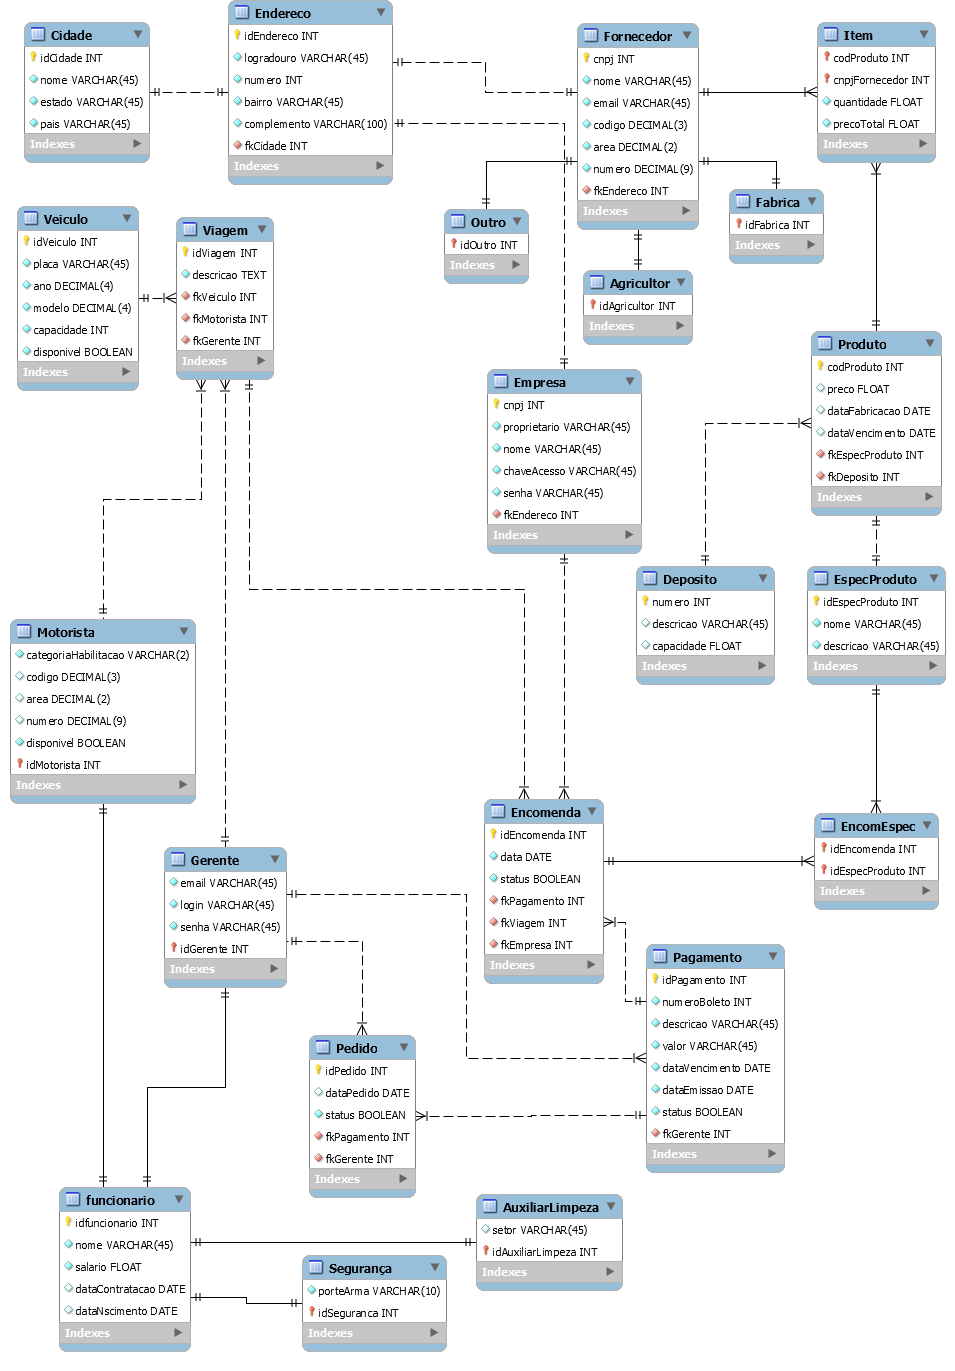
\includegraphics[scale=0.5]{modelo-relacional.png}
  \label{figRotulo}
\end{figure}

\newpage
\section{Normalização}
\label{sect:normalizacao}
Nesta seção será descrito o processo de normalização a partir do modelo relacional obtido na última etapa descrita da seção anterior.

\begin{description}

\item Primeira Forma Normal (1FN):

Nesta etapa, são verificadas as presenças de atributos multivalorados e não-atômicos.

\textit{(b)} - Todos os atributos de todas as relações já são monovaloradas e atômicos.

Logo está na 1FN.

\item Segunda Forma Normal (2FN):

Nesta etapa, são verificados atributos que dependem parcialmente das chaves compostas das relações.

\textit{b} - Nenhuma relação possui chave composta, logo todos os atributos dependem integralmente de suas chaves correspondentes.

Logo está na 2FN.

\item Terceira Forma Normal (3FN):

Nesta última etapa, são verificados se os atributos não-chaves dependem de outros atributos não-chaves, em caso afirmativo cria-se novas relações.

\textit{b} - Os atributos dependem unicamente das suas chaves primárias em cada relação.

Logo está na 3FN.
\end{description}

\newpage
\section{Álgebra Relacional}
\label{sect:algebra}

Com base nas principais consultas definidas anteriormente na seção \ref{sect:principaisConsultas} é detalhado a seguir cada uma dessas consultas que estão organizadas abaixo da seguinte forma: titulo, descrição e resolução utilizando a Algebra Relacional.\\

\begin{enumerate}

\item \textbf{Listagem de encomendas a partir de uma data.} \\\\
\qquad \textbf{Descrição:} Nesta consulta atraves de uma data especificado pelo usuário do sistema, é listado todas as encomendas que tem data superior a data previamente especificada.\\\\
\qquad \textbf{Resolução de consulta:}\\
\qquad $\sigma _{(data > varData )}$ (Encomenda)\\

\item \textbf{Busca por fornecedores que ofertam um determinado produto.}\\\\
\qquad \textbf{Descrição:} Nesta consulta atraves de um determinado produto é listado todos os fornecedores que fornecem este determinado produto.\\\\
\qquad \textbf{Resolução de consulta:}\\
\qquad (Fornecedor * ($\pi _{(idFornecedor)}$ (Item * ($\pi _{(codProduto)}$ (Produto X ($\pi _{(idEspecProduto)}$ ($\sigma _{(nome=varNome)}$ (EspecProduto)))))))\\

\item \textbf{Listagem de pagamentos recebidos de empresas.} \\\\
\qquad \textbf{Descrição:} Nesta consulta atraves de um determinado item especificado pelo usuário do sistema, é verificado se este item está em algum depósito, caso esteja é listado os itens e o depósito em que ele está.\\\\
\qquad \textbf{Resolução de consulta:}\\
\qquad $\sigma _{(status="finalizado")}$ ($\sigma _{(idPagamento=fkPagamento)}$ (Pagamento X $\pi_{fkPagamento}$ (Encomenda)))

\item \textbf{Listagem de pagamentos realizados a fornecedores.} \\\\
\qquad \textbf{Descrição:} Nesta consulta é listado todos os pagamentos que a distribuidora de alimentos fez aos seus fornecedores.\\\\
\qquad \textbf{Resolução de consulta:}\\
\qquad $\sigma _{(status="finalizado")}$ ($\sigma _{(idPagamento=fkPagamento)}$ (Pagamento X $\pi_{fkPagamento}$ (Pedido)))\\

\item \textbf{Listagem de encomendas solicitadas.} \\\\
\qquad \textbf{Descrição:} Nesta consulta é listada todas as encomendas feitas por empresas clientes da distribuidora de alimentos.\\\\
\qquad \textbf{Resolução de consulta:}\\
\qquad $\sigma _{(status="executando")}$ (Encomenda)\\

\item \textbf{Busca e conseguentemente a listagem do endereço de entrega relativos á encomenda.
} \\\\
\qquad \textbf{Descrição:} Nesta consulta a partir de uma encomenda especificada pelo usuário será listado o endereço da empresa que solicitou está encomenda.\\\\
\qquad \textbf{Resolução de consulta:}\\
\qquad $\sigma _{(idEndereco=fkEndereco)}$ Endereco X ($\sigma _{(idEmpresa=fkEmpresa)}$ (Empresa X ($\sigma _{(idEncomenda=varEncomenda)}$ (Encomenda)))) \\

\item \textbf{Listagem de pedidos realizados.} \\\\
\qquad \textbf{Descrição:} Nesta consulta é listado todos os pedidos que a distribuidora de alimentos encaminhou para seus fornecedores.\\\\
\qquad \textbf{Resolução de consulta:}\\
\qquad $\sigma _{(status="concluido")}$ (Pedido) \\

\item \textbf{Consulta e listagem de veículos disponíveis.} \\\\
\qquad \textbf{Descrição:} Nesta consulta é listado todos os veículos disponiveis para realizar uma viagem.\\\\
\qquad \textbf{Resolução de consulta:}\\
\qquad $\sigma _{(status="disponivel")}$ (Veiculo) \\

\item \textbf{Consulta e listagem de motoristas disponíveis.} \\\\
\qquad \textbf{Descrição:} Nesta consulta é listado todos os motoristas disponiveis para realizar uma viagem.\\\\
\qquad \textbf{Resolução de consulta:}\\
\qquad $\sigma _{(status="disponivel")}$ (Motorista) \\

\item \textbf{Listagem de pedidos em andamento.} \\\\
\qquad \textbf{Descrição:} Nesta consulta é listado todos os pedidos que estão em andamento, ou seja, não foram concluidos.\\\\
\qquad \textbf{Resolução de consulta:}\\
\qquad $\sigma _{(status="executando")}$ (Pedido) \\

\end{enumerate}


\end{document}
